% !Mode:: "TeX:UTF-8"
\chapter{帧内无损编码优化算法}
\label{cha:c3}
本章从帧内无损编码的可优化方向的分析开始,引出本研究课题中提出的 3 个优化算法:
1) L 形迭代预测算法 L-IP;
2) L 形分块算法 L-BP;
3) 残差中值边缘检测算法 R-MED。
在具体描述所提出算法之前均先详细地分析了标准规定或 HM 参考软件中的实现方案,以与所提算法形成对比。最后在对各算法性能单独测试的基础上,给出联合算法的性能测试,以证明所提算法的有效性。

\section{帧内无损编码的可优化方向}
针对 H.26X 标准,可考虑优化多种编码工具使最终的编码效率提高,当将优化对象聚焦到帧内无损编码时,涉及到的可优化模块有:帧内预测模块、熵编码模块以及贯穿编码过程的率-失真优化模块。本课题中提出的 3 个优化算法是在深入分析帧内预测过程及率-失真优化过程后提出的。

对帧内预测过程进行分析。H.26X 的帧内预测是基于块结构进行的,在 H.265 中最小的预测单元大小为 4x4,但针对视频图像中纹理丰富的区域 4x4 大小仍显得有些不足。出于计算复杂度的考虑,H.26X 标准暂时难以跳出块预测的框架,因此寻找更为精准的预测方式是一个可行的优化方向。
块结构的预测准确度仍不够高的原因在于部分被预测点距离参考点的空间距离过大,基于此本课题中提出了 L 形迭代预测算法,在保持整体帧内预测流程仍是块结构的情况下将所有待预测点与参考点的距离缩短到了 1 单位。

对率-失真优化中的编码单元分割过程进行分析。为了同时在图像中的平缓区域和细节丰富区域得到良好的编码效率,H.26X 在 RDO 过程中会进行搜索,自适应地确定编码块的尺寸,即在平缓区域用较大的块进行编码,在细节丰富的区域划分出多而小的编码块进行编码。
在 H.265 中,帧内预测部分采用基于四叉树的循环分层结构,即对于一个 2Nx2N 大小的 CU,PU 可选择的模式只有两种:划分为 4 个 NxN 或保留 2Nx2N。仅能 2 选 1 的划分模式难以满足图像视频中复杂多变的纹理的编码需求,因此提供更多可选的划分模式是一个可行的优化方向。
基于此本课题中提出了一种非对称的 L 形分块算法,使 RDO 过程可以搜索更多的分块可能性。

对无损模式下帧内预测的残差进行分析。H.26X 中基础的无损编码是通过简单地跳过变换、量化和环路后处理等可能引入数值失真的步骤实现的\upcite{BypassImprovingSCC}。由于缺少了变换这一将数值能量集中的步骤,熵编码面临的压力剧增,既耗时又无法得到理想的编码效率。
但也可以注意到此时待编码数据不再是变换域系数而是预测残差,因此其仍具有空间域的物理意义。
通过进一步分析,发现无损模式下的待编码系数具有不同于自然图像的特殊的空间结构相关性,表现为含有丰富的边缘特征,因此利用待编码系数的特性,设法对其做二次处理使更有利于熵编码是一个可行的优化方向。
基于此本课题中提出了残差中值边缘检测算法 R-MED,对无损模式下的待编码系数进行再处理得到一组能量大幅降低的新待编码系数,以降低熵编码的压力提高整体编码效率。

后文将先后对上述 3 个可优化方向做进一步的分析,并详细描述、测试所提出的算法。

\section{帧内无损编码的预测过程优化}
H.26X 的帧内无损编码方案中,预测过程的准确度直接决定了最终待编码系数的能量高低,因此设法优化预测过程使预测残差尽量降低是一个有效的优化方案。帧内预测以块为单位的特性导致其预测结果在距离参考点远的地方误差大,本节将针对该缺陷进行分析和优化。

\subsection{帧内预测过程分析}
\label{cha:IntraPredDetail}
以 H.265 中亮度分量的预测策略为例进行分析。每个帧内亮度预测单元均可选择 35 种预测模式进行处理,包括 33 种角度模式和 2 种平滑模式(DC 模式、Planar 模式)。角度模式进行预测的核心思想是图像中距离相近的像素点在数值上也大概率相近,这种数值相近的规律有可能发生在任意方向上,因此 H.265 规定了 33 个角度以适应图像中不同方向的纹理,如图 \ref{fig:IntraAngModeOverview} 所示。
\begin{figure}[hbt]
    \centering
    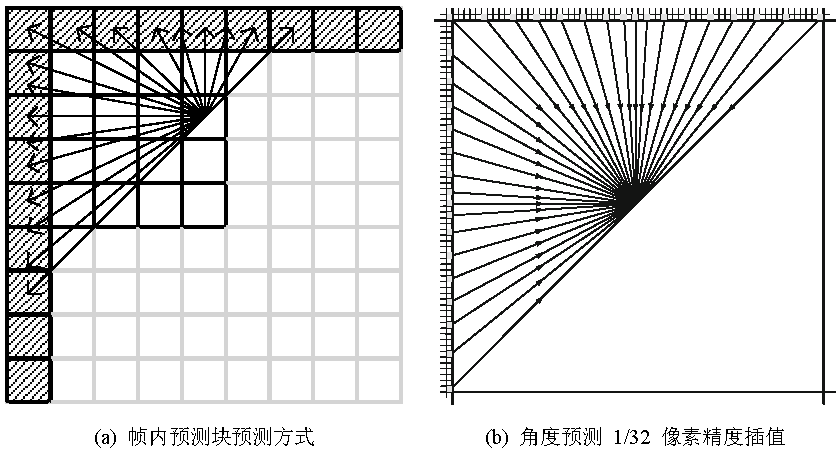
\includegraphics{IntraAngModeOverview.pdf}
    \caption{H.265 帧内预测角度模式}
    \label{fig:IntraAngModeOverview}
\end{figure}
\begin{figure}[hbt]
    \centering
    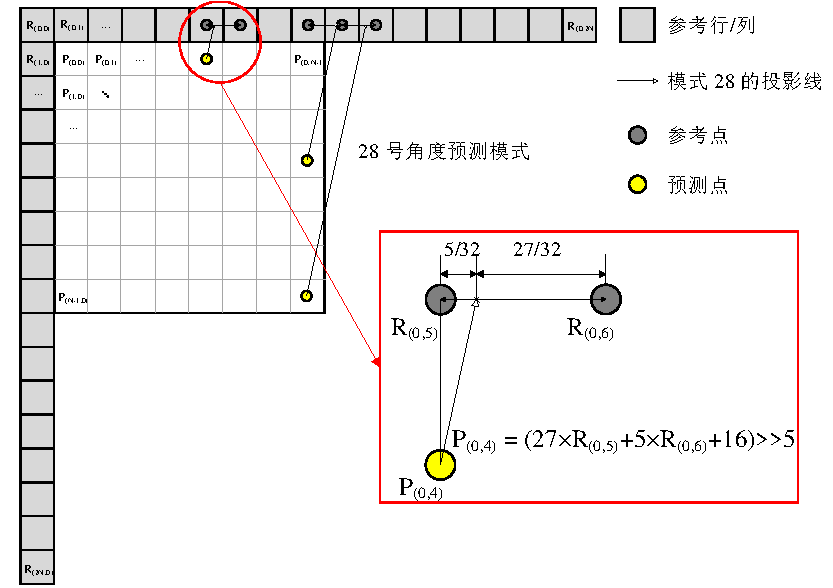
\includegraphics{Projection1_32Precision.pdf}
    \caption{H.265 角度预测 1/32 精度投影}
    \label{fig:Projection1_32Precision}
\end{figure}
显然可选择的方向越多越有可能得到准确的预测值,例如 H.266 中将可选的方向增加到了 65 种。角度预测的过程可以直观地理解为:使用待预测块左侧一列与上侧一行的参考点进行插值与投影。值得一提的是确定投影角度、插值时的权重分配均是以 1/32 像素精度进行的。坐标 $(x,y)$ 处的预测值 $P_{(x,y)}$ 的计算方式如下式: 
\begin{equation}
    P_{(x,y)}=((32-w)R_{(0,i)}+wR_{(0,i+1)}+16)>>5
    \label{equ:IntraProjection}
\end{equation}
其中 $R_{(0,i)}$ 与 $R_{(0,i+1)}$ 表示从待预测点投影到参考行、列时投影点左右的参考点数值,$w$ 用于控制权重分配,精度为 1/32,投影点距离 $R_{(0,i+1)}$ 越近 $w$ 越大。图 \ref{fig:Projection1_32Precision} 展示了 28 号角度预测模式下的投影与计算。

图 \ref{fig:IntraProjection} 展示了一个 8x8 大小的 PU 经过 H.265 的 35 种帧内预测方式后分别得到的预测结果。参考点取值波动极大,说明该待预测块附近很可能是纹理丰富的区域,因此从不同角度进行投影后得到的预测结果也呈现出丰富的边缘信息。
\begin{figure}[hbt]
    \centering
    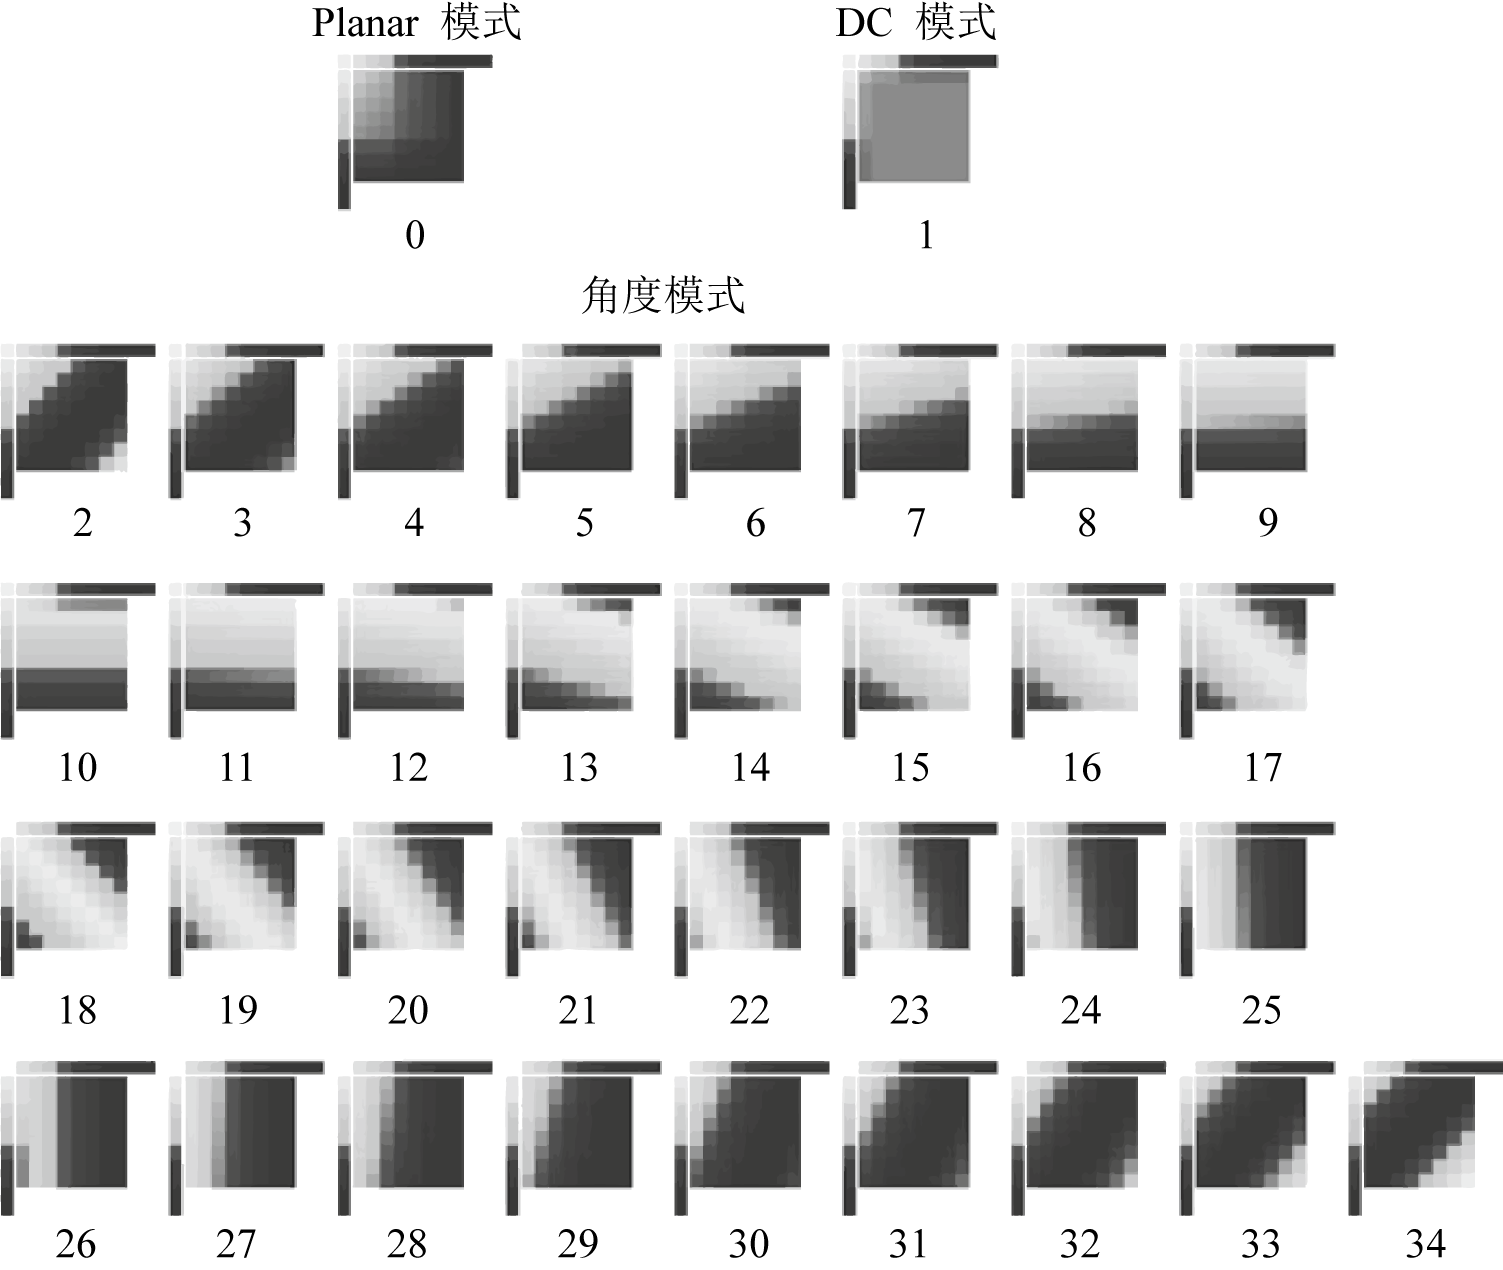
\includegraphics{IntraProjection.png}
    \caption{H.265 帧内预测结果示例}
    \label{fig:IntraProjection}
\end{figure}

最后,帧内预测过程还包含缺失参考点的填补方法、参考点的滤波策略和模式信息的编码方案等重要细节,但与将要提出的优化算法并无直接关系,暂不详述。在充分理解 H.26X 帧内预测的物理意义及预测过程后,下一节将分析其存在的缺陷并提出改进算法。

\subsection{L 形迭代预测算法}
\begin{figure}[hbt]
    \centering
    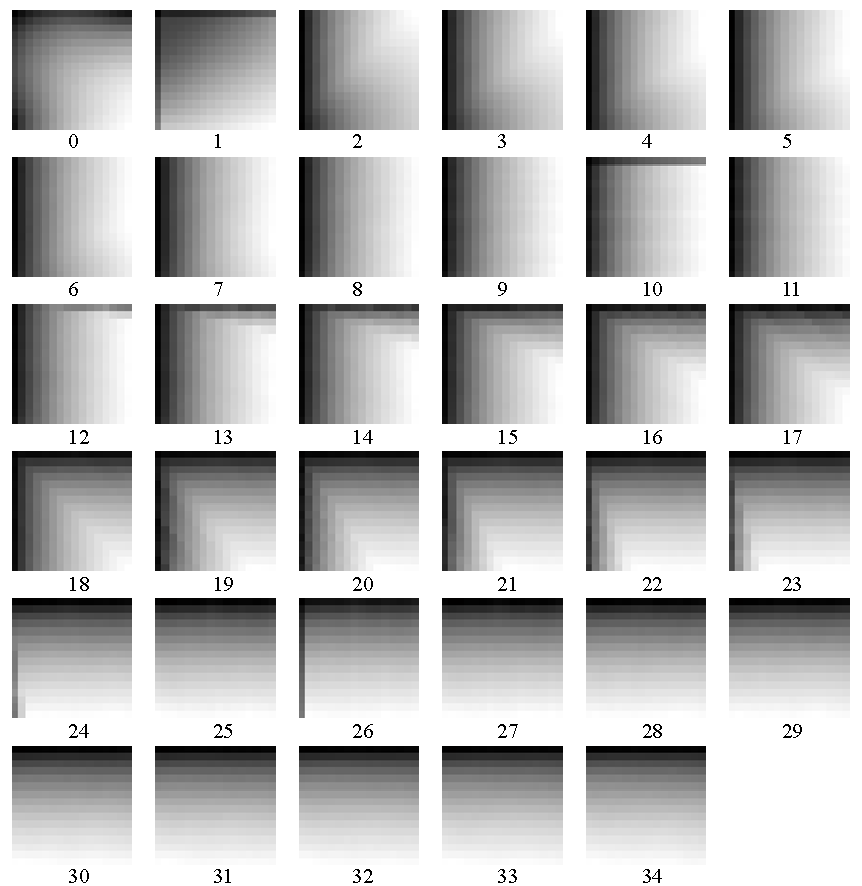
\includegraphics{ResidualVisible.pdf}
    \caption{H.265 帧内预测所有模式残差分布可视图}
    \label{fig:ResidualVisible}
\end{figure}
显然,距离参考行、列越远的待预测点越有可能得到误差大的预测值,这是自然图像朴素的特性决定的。出于研究的严谨性,可通过统计大量预测单元的残差分布来验证这一结论\upcite{ResidualVisible}。图 \ref{fig:ResidualVisible} 是 16x16 大小的预测单元,在所有 35 种帧内预测模式下产生的残差分布可视图,统计的对象来自 JCT-VC 推荐的 H.265 测试序列\upcite{HEVCCommonTestConditionsCTC}中的 $Traffic/Kimono/BasketballDrill/FourPeople$ 4 个序列的第一帧。图中颜色越深表示残差幅值越小即预测准确,反之颜色越淡表示预测越不准确。

分析图 \ref{fig:ResidualVisible} 的残差分布可得 2 条结论:1) 预测值的不准确性随着被预测点与参考点的距离增大而提升。换句话说,靠近参考点的待预测点能被准确地预测,较远区域的待预测点得到的预测效果差。这一现象是空间相关性随着预测距离增大而衰减造成的;2) 不同的预测模式下,靠近参考点的边界区域的预测准确度变化很大。观察图可以发现,模式 2\textasciitilde9 中左侧边界的预测准确度远高于上侧边界,这是由于模式 2\textasciitilde9 的预测过程中用到更多的左侧参考点,这些参考点十分靠近左边界。相反地,模式 27\textasciitilde34 的预测过程中用到更多的上侧参考点,因此表现为上侧边界的预测准确度高。

基于上述分析,为了对抗帧内预测中远离参考点的区域预测效果差的缺陷,本课题提出了 L 形迭代预测算法 L-IP。L-IP 的核心思想是将二维待预测块分割为一系列一维 L 形($\ulcorner$ 形)区域

\subsection{算法性能测试与分析}


\section{帧内无损编码的分块过程优化}

\subsection{帧内分块决策过程分析}

\subsection{L 形分块算法}

\subsection{算法性能测试与分析}


\section{帧内无损编码的待编码系数再处理}

\subsection{帧内预测残差分析}


\subsection{残差中值边缘检测算法}

\subsection{算法性能测试与分析}


\section{联合算法性能测试与分析}

\section{本章小结}